\documentclass[class=report, crop=false, 12pt,a4paper]{standalone}
\usepackage{enumitem}
\usepackage{gensymb}
\usepackage{siunitx}
\usepackage{graphicx}
\sisetup{detect-all}
\begin{document}
\subsection{Microstructures}
A higher level of structure visible using optical microscopy (even eyes) feature sizes (e.g. grains) in \si{\micro\meter} - \si{\milli\meter}. We see grains, grain boundaries, porosity and phases. Phase is a separately identifiable 'part' of a microstructure. In many materials often two or more phases exist. Single phase materials also occur e.g. pure substances. Type and quantity of phases present will affect the mechanical properties. We also need to consider the way they are arranged.

To explain what a phase 'is' we need to consider structures within grains. They are inevitable crystalline and possess long range order. There is a three dimensional periodicity and 14 separate ways of arranging points in space periodically. These are called lattices. A lattice (space lattice) is an array of points with identical surroundings that if repeated will create a crystal - lego brick. A lattice plus a motif creates a crystal structure.
\begin{figure}
  \centering
  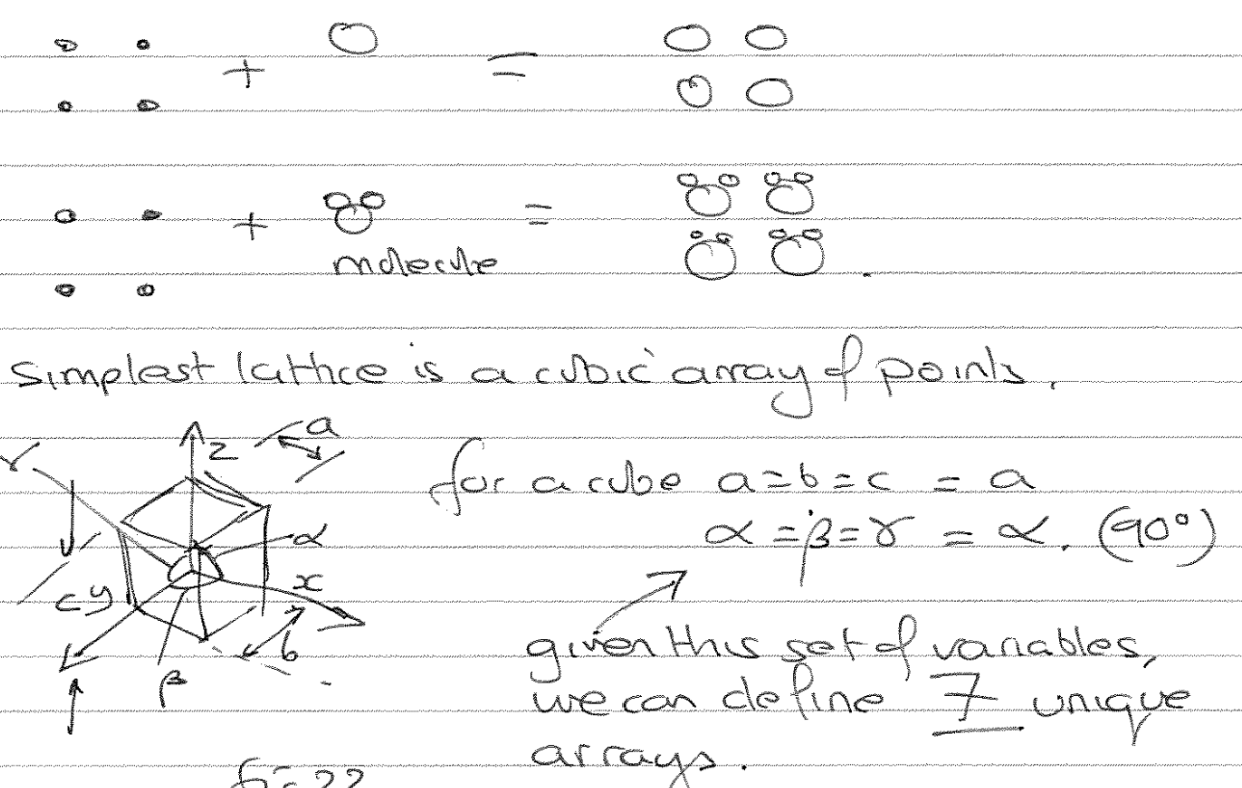
\includegraphics[width = 0.8\textwidth]{../img/latticeStructure}
  \caption{Lattice structure.}
\end{figure}
However there are another seven variants which contain additional 'points' inside or on a surface of the polygon. We have 14 Bravais lattices. All crystalline materials will exist in one of these forms. Atoms or molecules 'hang' on the lattice points and crystal structure strongly determine properties.

Common engineering metals exist in three main crystal structures.
\begin{enumerate}[noitemsep]
  \item Face centred cubic FCC. E.g. Cu, Al, Au, Ag, Pb, Ni, (Fe above 910 \si{\celsius} and below 1400 \si{\celsius}).
  \item Body centred cubic BCC. E.g. Fe , V, Mo, Cr, W.
  \item Hexagonal close packed HCP. E.g. Mg, Be, Zn, Cd, Co.
\end{enumerate}
Some elements can exist in different forms depending on temperature and pressure. E.g. Fe
\begin{enumerate}
  \item BCC up to 910 \si{\celsius} $\alpha$ (ferrite).
  \item FCC 910-1400 \si{\celsius} $\gamma$ (austentite).
  \item BCC 1400-1540 (melting point) $\delta$ ($\delta ferrite$).
\end{enumerate}
This is an example of allotropes.
\subsection{Atomic packing and crystal structure}
For many metals, the atoms are arranged in close packed planes, or close packed directions. assume an array of CP planes.
\begin{figure}
  \centering
  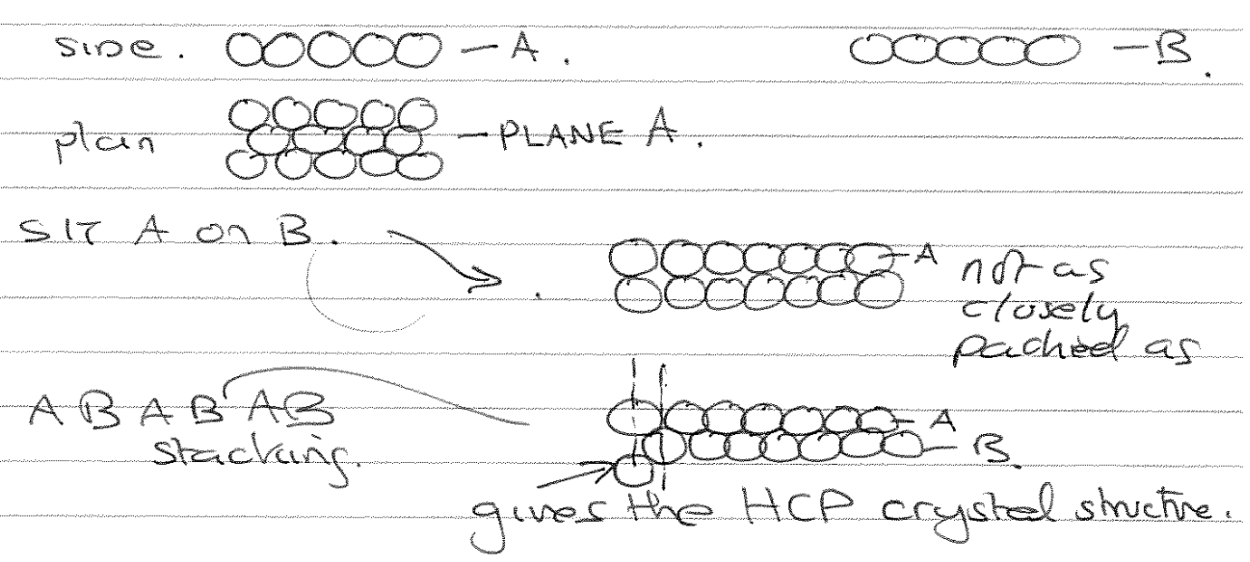
\includegraphics[width = 0.8\textwidth ]{../img/CPStructure}
\end{figure}
\end{document}